\documentclass[
    headings=optiontotocandhead,% Erweiterung für das optionale Argument der
                                % Gliederungsbefehle aktiviert.
    twoside,
    numbers=noenddot,% Keine Punkte am Ende der Gliederungsnummern und davon
                     % abgeleiteten Nummern
    toc=flat, %Flache TOC --- kann man anpassen (auskommentieren)
    12pt, % Schriftgröße 
    titlepage, % es wird eine Titelseite verwendet 
    parskip=full, % Abstand zwischen Absätzen (ganze Zeile) 
    listof=totoc, % Verzeichnisse im Inhaltsverzeichnis aufführen 
    listof=flat, % mehr Abstand für grosse Zahlen
    numbers=noenddot, % kein Punkt am Ende bei Nummern 
    %%enlargefirstpage,% Gibt es bei scrartcl nicht!!!!
    bibliography=totoc, % Literaturverzeichnis im Inhaltsverzeichnis aufführen 
    %index=totoc, % Index im Inhaltsverzeichnis aufführen 
    %captions=tableheading, % Beschriftung von Tabellen für Ausgabe oberhalb
            % der Tabelle formatieren 
    %draft % Status des Dokuments (final/draft) draft hinzufügen zum anziegen 
    %%der zeilen ende
    a4paper,DIV=14,
    BCOR=15mm,
    % captions=tablesignature,
]{scrbook}


\setcounter{secnumdepth}{3}

\usepackage[T1]{fontenc}
\usepackage[utf8]{inputenc}

\usepackage[english, ngerman]{babel} % your native language must be the last one!!

\usepackage{lastpage}
\usepackage{listings}
\usepackage{blindtext}

%% Aufzählungen nicht so weit einrücken
\usepackage[inline]{enumitem}
%\setitemize{leftmargin=*} 
% Listen etwas wenige einrücken, erfordert enumitem
\setitemize{leftmargin=*}

\usepackage{lmodern}
\usepackage{xspace}
\usepackage{graphicx}

%%? \usepackage{textcomp}
\usepackage[hyphens]{url}
%%? \usepackage{graphicx}
\usepackage[numbers]{natbib}
\PassOptionsToPackage{normalem}{ulem}
\usepackage{ulem}

\usepackage{needspace}

\setlength\partopsep{0.5ex}%schoenere Listen
\usepackage[bottom]{footmisc}%fussnote ganz unten

\usepackage[]{microtype}
\UseMicrotypeSet[protrusion]{basicmath} % disable protrusion for tt fonts

\usepackage{multirow}   % Allows table elements to span several rows.
\usepackage{booktabs}   % Improves the typesettings of tables.
\usepackage{subcaption} % Allows the use of subfigures and enables their referencing.
\usepackage[ruled,linesnumbered,algochapter]{algorithm2e} % Enables the writing of pseudo code.
\usepackage[usenames,dvipsnames,table]{xcolor} % Allows the definition and use of colors. This package has to be included before tikz.
\usepackage{nag}       % Issues warnings when best practices in writing LaTeX documents are violated.
\usepackage{todonotes} % Provides tooltip-like todo notes.

\usepackage{color}
\usepackage[binary-units]{siunitx}
\usepackage{longtable}
%% for pandoc2 images
\makeatletter
\def\maxwidth{\ifdim\Gin@nat@width>\linewidth\linewidth\else\Gin@nat@width\fi}
\def\maxheight{\ifdim\Gin@nat@height>\textheight\textheight\else\Gin@nat@height\fi}
\makeatother
% Scale images if necessary, so that they will not overflow the page
% margins by default, and it is still possible to overwrite the defaults
% using explicit options in \includegraphics[width, height, ...]{}
\setkeys{Gin}{width=\maxwidth,height=\maxheight,keepaspectratio}

%% bessere Suche im PDF
\input{glyphtounicode}
\pdfgentounicode=1
%%%%%%%%%%%%%%%%%%%%%%%%%%%%%%%%%%%%%%%%%%%%%%%%%%%%%%%%%%%%%%%%%%%%%%%%%%%%%%%%%%

%  Kopf und Fußzeilen -- links und rechts verschieden 
\newcommand{\kopfseitenummer}{{\bfseries \thepage}}
\newcommand{\kopfkapl}{{\bfseries\leftmark}}
\newcommand{\kopfkapr}{{\bfseries\rightmark}}
\newcommand{\kopfbild}{\voffset7mm
\includegraphics[width=25mm]{HTL3RLogoRGB}}
\newcommand{\kopfHTL}{Höhere Technische Bundeslehranstalt Wien 3, \\Rennweg 	Abteilung für Informationstechnologie}

\usepackage[automark,headsepline,footsepline,plainfootsepline]{scrlayer-scrpage}
%\automark[chapter]{chapter}% Eventuell wenn doppelseitig
\setkomafont{pageheadfoot}{\normalcolor\footnotesize\scshape}
\setkomafont{pagenumber}{\normalfont\normalsize}
\clearpairofpagestyles
\ihead{\headmark}
\ohead{\kopfbild}
\ofoot{\pagemark}
\ModifyLayer[addvoffset=-.6ex]{scrheadings.foot.above.line}% Linie verschieben
\ModifyLayer[addvoffset=-.6ex]{plain.scrheadings.foot.above.line}% Linie verschieben
\setlength{\headheight}{32pt}

% alle Seiten mit Kopfzeile
\renewcommand{\chapterpagestyle}{scrheadings}

%% Kapitel - aufwändige Kapitelüberschriften
%Options: Sonny, Lenny, Glenn, Conny, Rejne, Bjarne, Bjornstrup
%\usepackage[Bjornstrup]{fncychap}
% Alternative: 
%\usepackage{titlesec} 

% Verzeichnisse - aufwändiger
%\usepackage{tocloft}

%% Code Beispiele
%% eine Variante 
\usepackage{listings} 
\renewcommand{\lstlistingname}{\inputencoding{utf8}Listing}
%% andere Variante
%\usepackage{minted}
%\setminted{
%  linenos,
%  frame=lines,
%  framesep=2mm,
%  breaklines=true
%}
% Beispiel
%\begin{listing}[H]
%\begin{minted}{bash}
%...
%\end{minted}
%\caption{Beschreibung}
%\end{listing}
%% dritte Variante 
% mit/für pandoc

%% should be last packages
\usepackage{scrhack}

%% sollte das letzte Package sein
\usepackage[unicode=true,
 bookmarks=true,bookmarksnumbered=false,bookmarksopen=false,
 breaklinks=true,pdfborder={0 0 0},backref=false,colorlinks=false]
 {hyperref}
\urlstyle{same} % don't use monospace font for urls

%% for pandoc
\providecommand{\tightlist}{%
  \setlength{\itemsep}{0pt}\setlength{\parskip}{0pt}}

% Auch Fußnoten bündig ausrichten
\deffootnote[]{1em}{1em}{\textsuperscript{\thefootnotemark\ }}
%% setup
\sloppy % weniger Meldungen
\voffset7mm % etwas nach unten

%% schöner: 10000 -- gar keine, 1000 als Mittelweg
\clubpenalty = 1000 % Schusterjungen verhindern
\widowpenalty = 1000 % Hurenkinder verhindern
\displaywidowpenalty = 1000 

%%%%%%%%%%%%%%%%%%%%%%%%%%%%%%%%%%%%%%%%%%%%%%%%%%%%%%%%%%%%%%%%%%%%%%%%%%%%%%%%%%

\begin{document}

\title{Diplomarbeit}
\begin{titlepage}
\begin{minipage}[b]{1\columnwidth}
\parbox[b]{50mm}{
\includegraphics[width=45mm]{HTL3RLogoRGB}}
\hfill
\parbox[b]{130mm}{\footnotesize \textsc{Höhere Technische Bundeslehranstalt} Wien 3, Rennweg\\
IT \& Mechatronik\\
\\
HTL Rennweg :: Rennweg 89b\\
A-1030 Wien :: Tel +43 1 24215-10 :: Fax DW 18
}\\
\mbox{}
\end{minipage}

\vspace{1cm}


\begin{center}
\textbf{\LARGE{}Laborprotokoll}{\large{}}\\ 
{\large{}\vspace{15mm}
 } \textbf{\large{Kubernetes, VEEAM und PRTG}}\\
 \vspace{15mm}
 ausgeführt an der\\
 Höheren Abteilung für Informationstechnologie\\
 der Höheren Technischen Lehranstalt Wien 3 Rennweg\\
 \vspace{1cm}
 im Schuljahr 2019/2020\\
 \vspace{1cm}
 durch\\
 \vspace{0.5cm}
\textbf{\large{}Leon Kirschner}\\
\textbf{\large{}Michael Kudler}\\

\par\end{center}{\large \par}

\begin{center}
  \vspace{15mm}
   \normalsize im Auftrag von\\
   \vspace{0.5cm}
  DI Bernhard Nickel\\ 
  \par\end{center}

\begin{center}
\vspace{5mm}
Wien, \today 
\par\end{center} 
 
\end{titlepage}

\cleardoublepage{}
\tableofcontents{}
\cleardoublepage{}

\mainmatter

\chapter{Containerorchestrierung mit Kubernetes}
\hypertarget{aufgabenstellung}{%
\section{Aufgabenstellung}\label{aufgabenstellung}}

Die Idee des Projektes ist es einen Kubernetes Cluster auf 3 VMS zu
deployen und die Möglichkeiten die dadurch entstehen zu erkunden.

Ein optionales Ziel ist es, diese Infrastruktur auf eine Web-Applikation
mit Anbindung einer Datenbank anzuwenden und Aktivitäten zu überprüfen.

\hypertarget{kubernetes}{%
\subsection{Kubernetes}\label{kubernetes}}

Kubernetes ist ein Open-Source Orchestrierungs Tool, das dazu dient
Container automatisiert Bereitzustellen und zu verwalten.

\begin{quote}
Der Name Kubernets kommt aus dem griechischen und steht für Steuermann.
\end{quote}

Wir verwenden in unserem Projekt \href{https://www.docker.com/}{Docker}
als Container Runtime.

\hypertarget{aufbau-und-architektur}{%
\subsubsection{Aufbau und Architektur}\label{aufbau-und-architektur}}

\begin{figure}
\centering
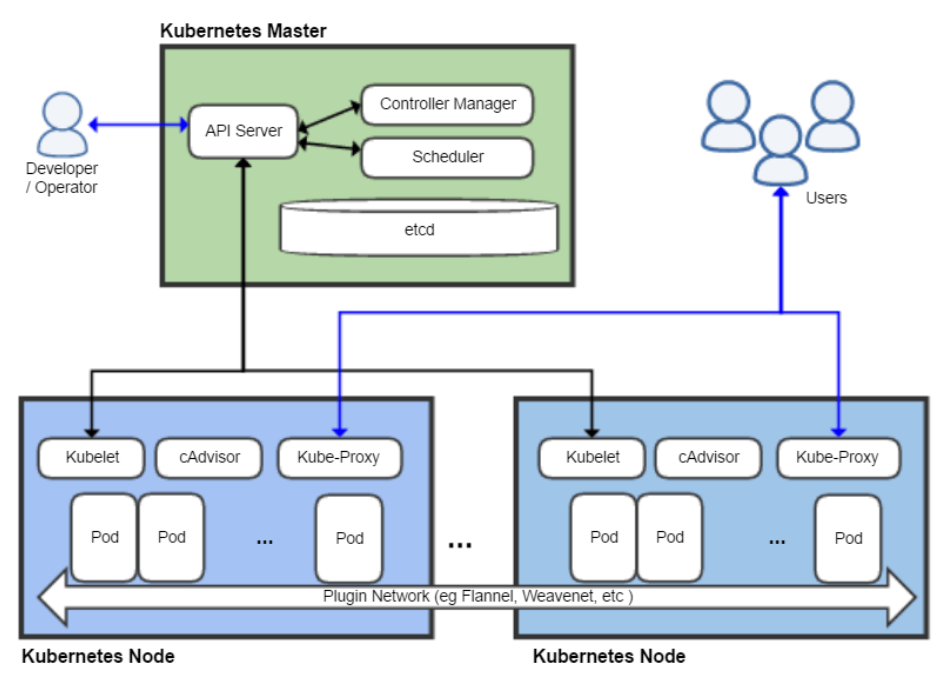
\includegraphics[width=0.8\textwidth]{./images/kuber.png}
\caption{Kubernetes Architektur}
\end{figure}

Der Vorteil bei Kubernetes liegt darin, dass es \emph{Pods}
orchestriert. Sie stellen die kleinstmögliche steuerbare Einheit im
Kubernetes Universum dar. Sie laufen auf \emph{Nodes} - also VMs oder
physischen Maschinen). Ein Pod kann einen oder mehrere Container
beinhalten.

Die Architektur ist auf dem Master-Slave System aufgebaut.

Der Master ist die \emph{Control Plane}, auf ihr wird Inventur über alle
Objekte in einem Cluster geführt. Der Master steuert außerdem alle
Slaves (Minions). Wir haben in unserem Fall nur einen Master-Node. Es
können aber auch - zwecks Redundanz - mehre Master-Nodes in einem
Kubernetes Cluster konfiguriert werden.

Auf jedem Minion muss zusätzlich auch die zu verwendente
Container-Runtime installiert werden.

\hypertarget{installation}{%
\newpage
\section{Installation}\label{installation}}

\hypertarget{validierung-bevor-es-losgeht}{%
\subsection{Validierung bevor es
losgeht}\label{validierung-bevor-es-losgeht}}

Bei jedem Node (VM oder physische Maschine), die im Cluster verwendet
werden soll, müssen sich folgende Eigenschaften unterscheiden:

% \begin{longtable}[]{@{}ll@{}}
% \toprule
% Eigenschaft & Befehl zum Prüfen\tabularnewline
% \midrule
% \endhead
% MAC Adresse & \lstinline{!ip link!}\tabularnewline
% Produkt UUID & \lstinline{{!cat /sys/class/dmi/id product\_uuid!}}\tabularnewline
% \bottomrule
% \end{longtable}

Da wir für dieses Beispiel Debian 10 verwenden, müssen wir zusätzlich
noch iptables in den legacy-mode schalten.

\begin{lstlisting}[language=Bash]
update-alternatives --set iptables /usr/sbin/iptables-legacy
update-alternatives --set ip6tables /usr/sbin/ip6tables-legacy
update-alternatives --set arptables /usr/sbin/arptables-legacy
update-alternatives --set ebtables /usr/sbin/ebtables-legacy
\end{lstlisting}

\hypertarget{installation-1}{%
\newpage
\section{Installation}\label{installation-1}}

\hypertarget{docker}{%
\subsection{Docker}\label{docker}}

Als Container Runtime benutzen wir für dieses Beispiel Docker.

Zuerst müssen wir alle Dependencies von Docker installieren.

\begin{lstlisting}[language=Bash]
apt update
apt -y install apt-transport-https ca-certificates curl gnupg2 software-properties-common
\end{lstlisting}

Anschließend fügen für den offiziellen GPG-Key von Docker zu unserem
Package-Manager hinzu. Mit diesem Schlüssel sind die Packete signiert.

\begin{lstlisting}[language=Bash]
curl -fsSL https://download.docker.com/linux/debian/gpg | apt-key add -
\end{lstlisting}

Nun können wir die offiziellen Docker-Repositories hinzufügen.

\begin{lstlisting}[language=Bash]
add-apt-repository \
   "deb [arch=amd64] https://download.docker.com/linux/debian \
   $(lsb_release -cs) \
   stable"
\end{lstlisting}

Die Installation selbst ist nun ziemlich einfach.

\begin{lstlisting}[language=Bash]
apt-get update && apt-get install -y \
  containerd.io=1.2.10-3 \
  docker-ce=5:19.03.4~3-0~debian-$(lsb_release -cs) \
  docker-ce-cli=5:19.03.4~3-0~debian-$(lsb_release -cs)
\end{lstlisting}

Zu guter Letzt passen wir noch die Einstellungen für Docker an.

\begin{lstlisting}[language=Bash]
cat > /etc/docker/daemon.json <<EOF
{
  "exec-opts": ["native.cgroupdriver=systemd"],
  "log-driver": "json-file",
  "log-opts": {
    "max-size": "100m"
  },
  "storage-driver": "overlay2"
}
EOF

mkdir -p /etc/systemd/system/docker.service.d
\end{lstlisting}

Einen kleinen Restart brauchen wir noch.

\begin{lstlisting}[language=Bash]
systemctl daemon-reload
systemctl restart docker
\end{lstlisting}

Wie jeder gute IT-Admin werden verifizieren wir natürlich noch am Ende
die gelungene Installation.

\begin{lstlisting}[language=Bash]
docker version
\end{lstlisting}

Falls hier vernünftige Informationen angezeigt werden und keine
Fehlermeldung ist die Installation gelungen.

\hypertarget{kubernetes-1}{%
\subsection{Kubernetes}\label{kubernetes-1}}

Als nächsten Schritt installieren wir Kubernetes. Oder besser gesagt die
3 Services, aus denen unsere Kubernetes Installation bestehen wird.

\begin{itemize}
\tightlist
\item
  kubeadm
\item
  kubelet
\item
  kubectl
\end{itemize}

Dafür benutzen wir einen ähnlichen Ablauf, wie bei Docker. Der
Einfachheit halber ist nun nicht jeder Schritt kommentiert, sondern ein
fertiges Skript zu sehen.

\begin{lstlisting}[language=Bash]
apt-get update && sudo apt-get install -y apt-transport-https curl
curl -s https://packages.cloud.google.com/apt/doc/apt-key.gpg | sudo apt-key add -
cat <<EOF | sudo tee /etc/apt/sources.list.d/kubernetes.list
deb https://apt.kubernetes.io/ kubernetes-xenial main
EOF
apt-get update
apt-get install -y kubelet kubeadm kubectl
apt-mark hold kubelet kubeadm kubectl
\end{lstlisting}

Auch hier folgt natürlich wieder die Verifikation.

\begin{lstlisting}[language=Bash]
kubeadm version
kubelet --version
kubectl version
\end{lstlisting}

\hypertarget{erstellung-eines-clusters}{%
\newpage
\section{Erstellung eines Clusters}\label{erstellung-eines-clusters}}

\hypertarget{einstellungen}{%
\subsection{Einstellungen}\label{einstellungen}}

Ein kleiner Schritt hält uns noch vom Cluster ab: Wir müssen swap
abschalten.

\begin{lstlisting}[language=Bash]
swapoff -a
cp /etc/fstab /etc/fstab.orig
cat /etc/fstab.orig | grep -v 'swap' > /etc/fstab
\end{lstlisting}

Jetzt noch ein Reboot.

\begin{lstlisting}[language=Bash]
reboot 0
\end{lstlisting}

\hypertarget{kubeadm}{%
\subsection{Kubeadm}\label{kubeadm}}

Bevor man den Cluster installiert muss man sich für ein pod network
add-on entscheiden. Die Auswahl ist da groß, weswegen wir uns
schlichtweg für das beliebteste Add-On entschieden haben: Flannel

Auf unserem Master führen wir nun folgenden Befehl aus:

\begin{lstlisting}[language=Bash]
kubeadm init --pod-network-cidr=10.244.0.0/16
\end{lstlisting}

Mit den anderen Nodes können wir jetzt joinen. Den Befehl dafür finden
wir im Output von kubeadm init am Master.

\begin{lstlisting}[language=Bash]
kubeadm join 10.0.0.88:6443 --token <token> \
    --discovery-token-ca-cert-hash sha256:<hash>
\end{lstlisting}

\hypertarget{troubleshooting}{%
\newpage
\section{Troubleshooting}\label{troubleshooting}}

Bei der Verifizierung am Master mit
\lstinline{!kubectl get nodes!} kann es zu folgendem Fehler
kommen:

\begin{lstlisting}[language=Bash]
The connection to the server localhost:8080 was refused - did you specify the right host or port?
\end{lstlisting}

Das lässt sich mit den folgenden Befehlen beheben. (Credits an den
\href{https://github.com/kubernetes/kubernetes/issues/44665\#issuecomment-295216655}{GitHub
post von user csarora})

\begin{lstlisting}[language=Bash]
cp /etc/kubernetes/admin.conf $HOME/
chown $(id -u):$(id -g) $HOME/admin.conf
export KUBECONFIG=$HOME/admin.conf
\end{lstlisting} 

\chapter{Netzwerküberwachung mit PRTG}
Die Software PRTG\(\footnote{Früher Pässler Router Traffic Grapher}\)
der deutschen Firma Paessler GmbH bietet eine Vielzahl an Tools um
nahezu jede Komponente eines Netzwerks zu überwachen. Einige wichtige
Features bilden:

\begin{itemize}
\item
  Unterstützung aller gängige Agents: SNMP, WMI, SSH bzw. Agentless:
  SQL, Ping, REST APIs und viel mehr.
\item
  Maps und Dashboard: Intuitive Erstellung von Dashboards zur echtzeit
  Überwachung mit Live-Stausinformationen
\item
  Flexibler Alarm: PRTG alarmiert automatisch den Administrator, sobald
  Problem oder Anomalien entdeckt werden.
\end{itemize}

Paessler bietet mehrere Lizenzen an, die sich haupsächlich durch die
Anzahl der Sensoren unterscheiden. Angefangen bei 1.300€ mit 500
unterstützen Sensoren für kleine Unternehmen bis hin zu 12.500€ mit
unbegrenzten Sensoren für größere Unternehmen, ist für jeden was dabei.
Zu Testzwecken stellt Paessler jedem eine 30 Tage Testversion zur
Verfügung.

\hypertarget{installation-erste-schritte}{%
\section{Installation \& Erste
Schritte}\label{installation-erste-schritte}}

Die Installation des Tools ist intuitiv und dauert nur wenige Minuten.
Nachdem PRTG heruntergeladen ist, wird die Software installiert und
automatisch gestartet. Es handelt sich hierbei um eine Webapplikation,
die über die IP-Adresse des Computers erreichbar ist und über jeden
Webbrowser erreichbar ist, der den Server erreichen kann.

\begin{figure}[!htb]
\centering
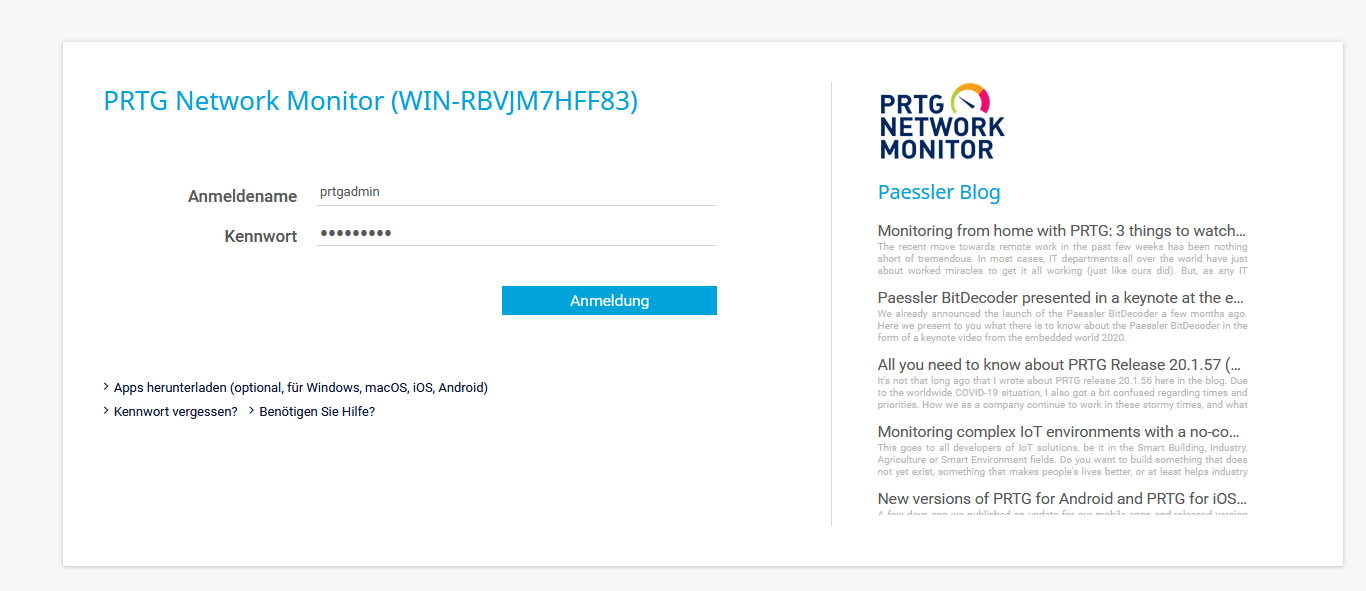
\includegraphics{./images/prtg_welcome.png}
\caption{PRTG Anmeldemaske}\label{prtg-anmeldemaske}
\end{figure}

Bevor man jedoch anfängt mit PRTF zu arbeiten, sollten einem einige
Begriffe geläufig sein. Eineer dieser Begriffe ist der Sensor. Sensoren
sind das um und auf der PRTG Network Monitor Software. Ein Sensor ist
ein Messpunkt, der einen \emph{Aspekt} auf einem Gerät überwacht.
Beispiele dafür wären CPU-Auslastung eines Servers oder die
Portauslastung eines Interfaces auf einem Switch. So ermöglichen eine
Vielzahl von Sensoren die Rundumüberwachung verschiedenster Geräte. Ein
Sensor schleust Daten in einen \emph{Kanal}. So hat der Ping Sensor die
Kanäle Latenz(ms), Paketverlust(\%), etc. .

\hypertarget{lab-uxfcberwachung-von-linux-und-windows-server}{%
\section{LAB: Überwachung von Linux und Windows
Server}\label{lab-uxfcberwachung-von-linux-und-windows-server}}

Das folgende Kapitel beschäftigt sich mit der Überwachung einer
einfachen Serverinfrastruktur.

\hypertarget{topologie}{%
\subsection{Topologie}\label{topologie}}

\begin{figure}[!htb]
\centering
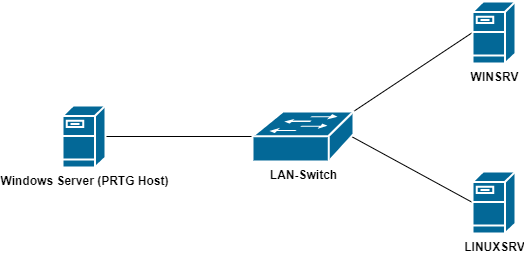
\includegraphics{./images/prtg_architektur.png}
\caption{PRTG LAB Architektur}
\end{figure}

Die Infrastruktur besteht aus drei Servern:

\begin{itemize}
\tightlist
\item
  Windows Server (PRTG Host): Der Monitoring Server
\item
  WINSRV: Windows Server
\item
  LINUXSRV: Linux Server mit einem Apache Server
\end{itemize}

\hypertarget{uxfcberwachung-linux-server}{%
\subsection{Überwachung Linux
Server}\label{uxfcberwachung-linux-server}}

Im ersten Schritt muss das Gerät registriert werden. Dazu im Reiter
\emph{Geräte} auf \emph{Gerät hinzufügen} klciken und einen Gruppe nach
belieben auswählen\$\textbackslash footnote\{Wir haben die Gruppe
\emph{Linux/ macOS / Unix} gewählt\}. Danach erscheint es in der
Geräteliste:

\begin{figure}[!htb]
\centering
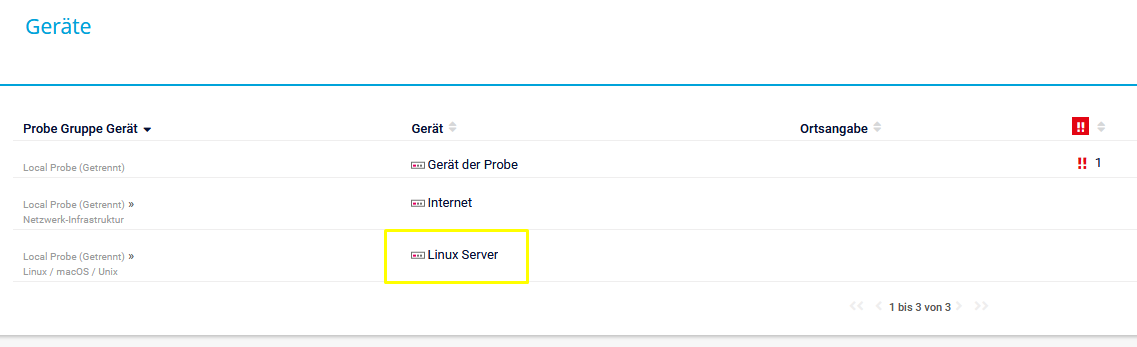
\includegraphics{./images/prtg_linux-server.png}
\caption{PRTG Gerät: Linux Server}
\end{figure}

Die Überwachung eines Linux Servers funktioniert meist Agentless. Es
muss also auf dem Zielgerät nichts installiert werden und
Informationsafrage findet über Protokolle wie SSH, HTTP oder SNMP statt.
Dementsprechend ist die Konfiguration von Sensoren für Linux System
ziemlich straight-forward. Nichtsdestotrotz mussten einige
Vorbereitungen getroffen werden:

\begin{enumerate}
\def\labelenumi{\arabic{enumi}.}
\item
  Open-SSH Server
  installieren\(\footnote{Meist vorinstalliert, bei uns (Linux Mint) jedoch nicht}\)
\item
  Apache Server installieren\(\footnote{apache2}\)
\end{enumerate}

\hypertarget{erster-sensor-ping}{%
\subsubsection{Erster Sensor: Ping}\label{erster-sensor-ping}}

Auf der Geräteseite des Linux Servers kann in der Sensorenbox via Klick
auf das ``+'' ein Sensor hinzugefügt werden.

\begin{figure}[!htb]
\centering
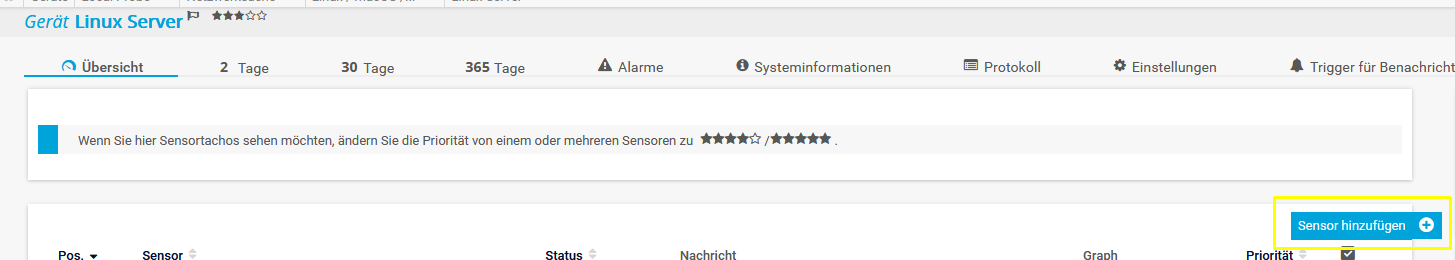
\includegraphics{./images/prtg_add_sensor.png}
\caption{PRTG Sensor hinzufügen}
\end{figure}

Im nächsten Schritt ist der gewünschte Sensortyp auszuwählen, in unserem
Fall Ping. Danach sind einige Paramter einzugeben, wir lassen sie auf
den Defaulteinstellungen. Nach einer kurzen Wartezeit, kann man sich mit
Klick auf den Ping Sensor eine Statistik über die abgesetzten Pings
anschauen.

\begin{figure}[!htb]
\centering
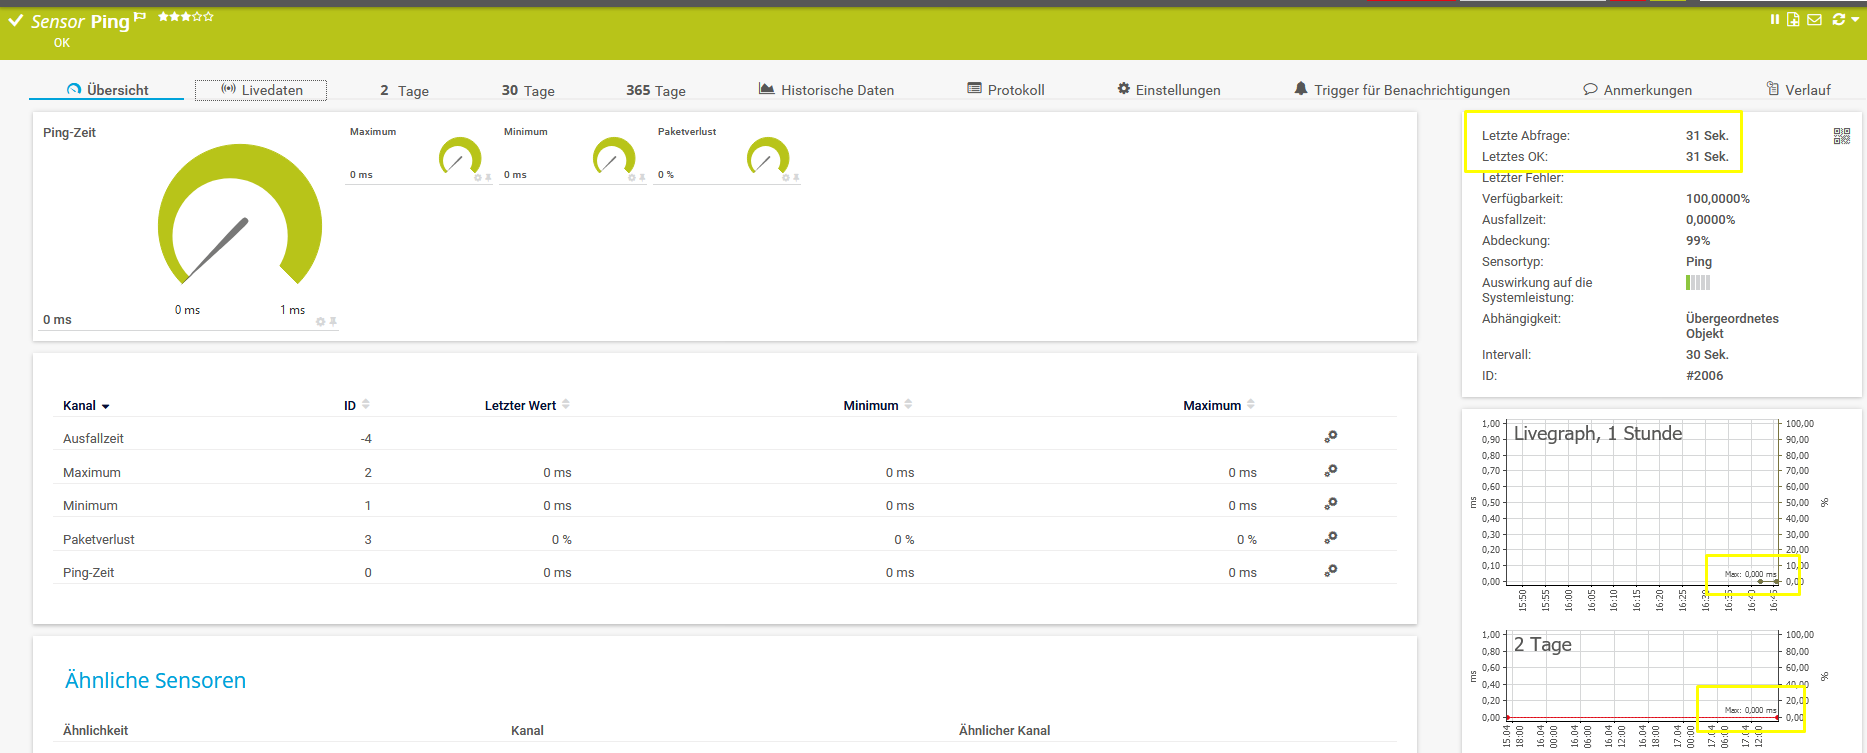
\includegraphics{./images/prtg_ping_statistik.png}
\caption{PRTG Sensor Statistiken}
\end{figure}

\hypertarget{apache-server-uxfcberwachen}{%
\subsubsection{Apache Server
überwachen}\label{apache-server-uxfcberwachen}}

Auf dem Linux Server wurde kurzerhand ein Apache Server installiert.
Über den HTTP Sensor lässt sich auch dieser ziemlich schnell und einfach
überwachen. Dazu dem selben Prozedere wie zuvor folgen.

\begin{figure}[!htb]
\centering
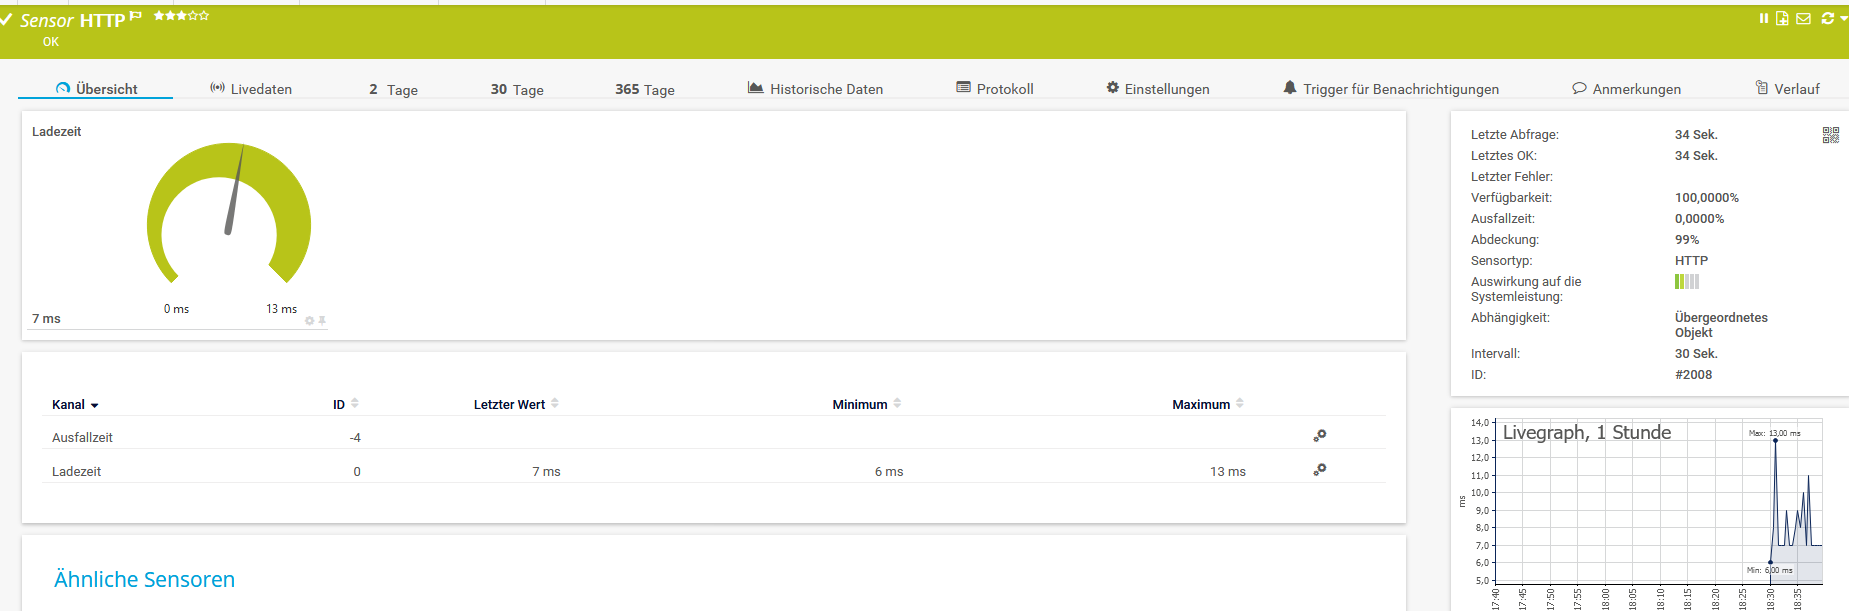
\includegraphics{./images/prtg_http.png}
\caption{PRTG Überwachung des Apache Serverss}
\end{figure}

Diesmal wollen wir allerdings eine Benachrichtigung erhalten, sobald der
Apache Server einen Fehler aufweist. Hierfür muss auf der Geräte Seite
unter dem Tab \emph{Trigger für Benachrichtigungen} ein neuer Trigger
hinzugefügt werden. In unserem Fall soll der Trigger nach 20 Sekunden
durchgehendem fehlerhaften Verhalten ein Ticket erstellt werden.

\begin{figure}[!htb]
\centering
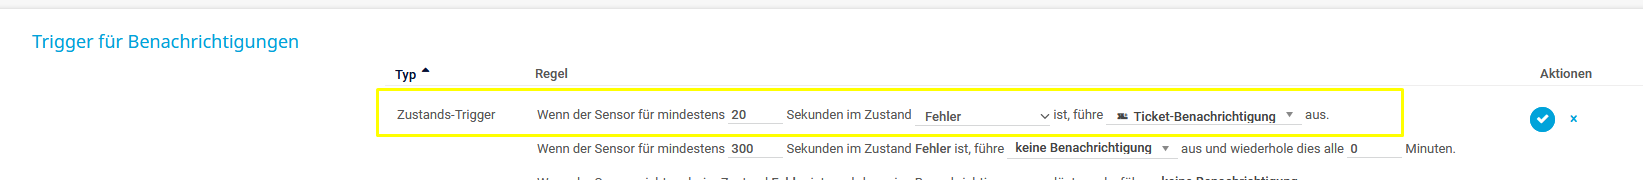
\includegraphics{./images/prtg_ticker.png}
\caption{PRTG Triggeraktion}
\end{figure}

Um zu testen wurde der Apache Server kurzerhand gestoppt und wie zu
erwarten wurde ein wenig später ein Ticket erstellt.

\begin{figure}[!htb]
\centering
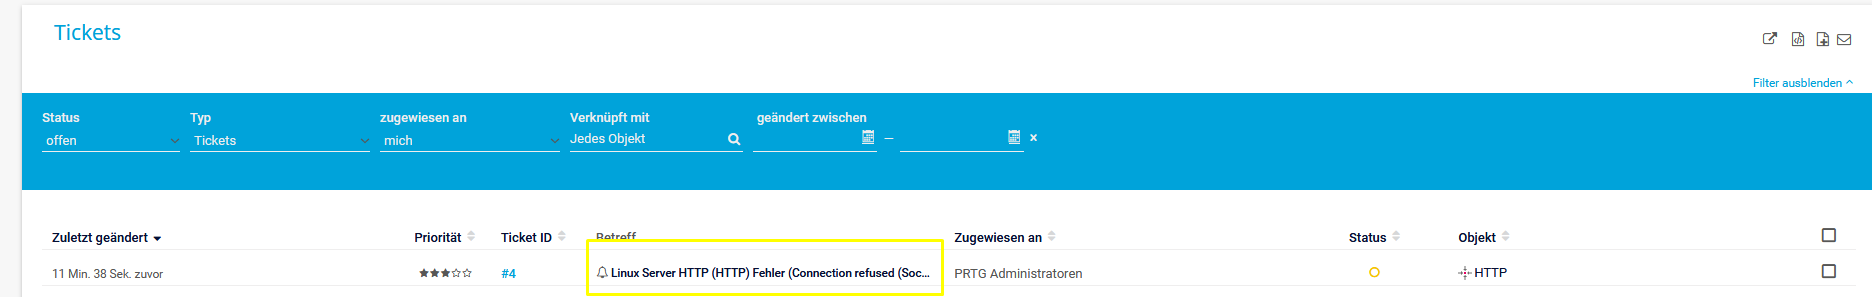
\includegraphics{./images/prtg-created-ticket.png}
\caption{PRTG Ticket}
\end{figure}

Mit einem Klick auf das Ticket können Details angezeigt werden
(Abbildung \ref{prtg-ticket}).

\begin{figure}[!htb]
\centering
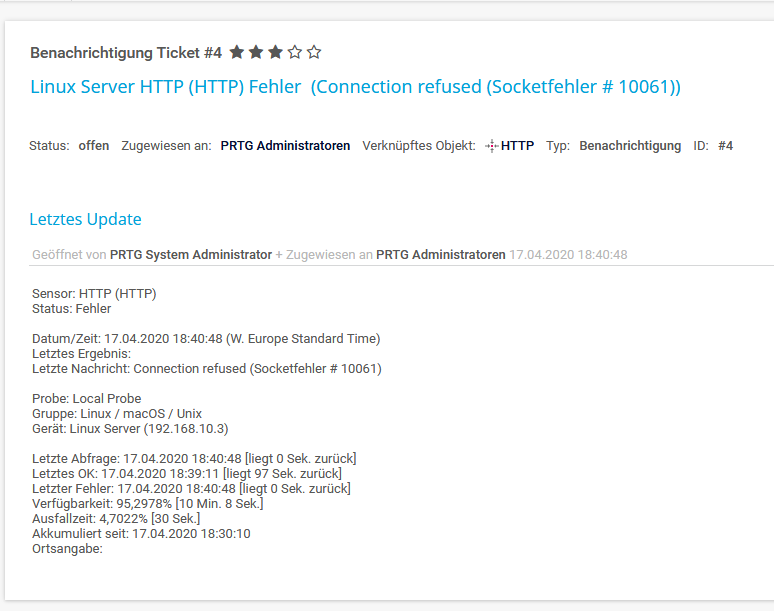
\includegraphics{./images/prtg-ticket-details.png}
\caption{PRTG Ticketdetails}\label{prtg-ticket}
\end{figure}

\hypertarget{erweiterte-sensoren}{%
\subsubsection{Erweiterte Sensoren}\label{erweiterte-sensoren}}

Um einen - meines Erachtens - recht außergewhönlichen Sensor zu
testen/implementieren. Wurde auf dem Linux Server mittels Flask und
Python eine REST-Api programmiert um den PRTG REST Sensor zu testen.

\begin{lstlisting}[language=Python]
from flask import Flask, jsonify

app = Flask(__name__)

@app.route("/")
def hellOWorld():
    return jsonify({"hallo" : "welt"})


if __name == 'main__':
    app.run(host='192.168.10.3', port=8080)
\end{lstlisting}

die mit REST API\(\footnote{noch in der BETA Version}\) Sensor überprüft
werden kann. Untr dem Reiter \emph{Historische Daten} kann man die
gesammelten Daten als CSV, kann man alle gesammelten Daten im CSV, XML
oder HTML exportieren um daraus z.B. Grafiken zu generieren. Zusätzlich
können Paremter wie der Zeitraum, das Durchschnittsinterval und die
gesammelten Kanäle angepasst werden.

\begin{figure}[!htb]
\centering
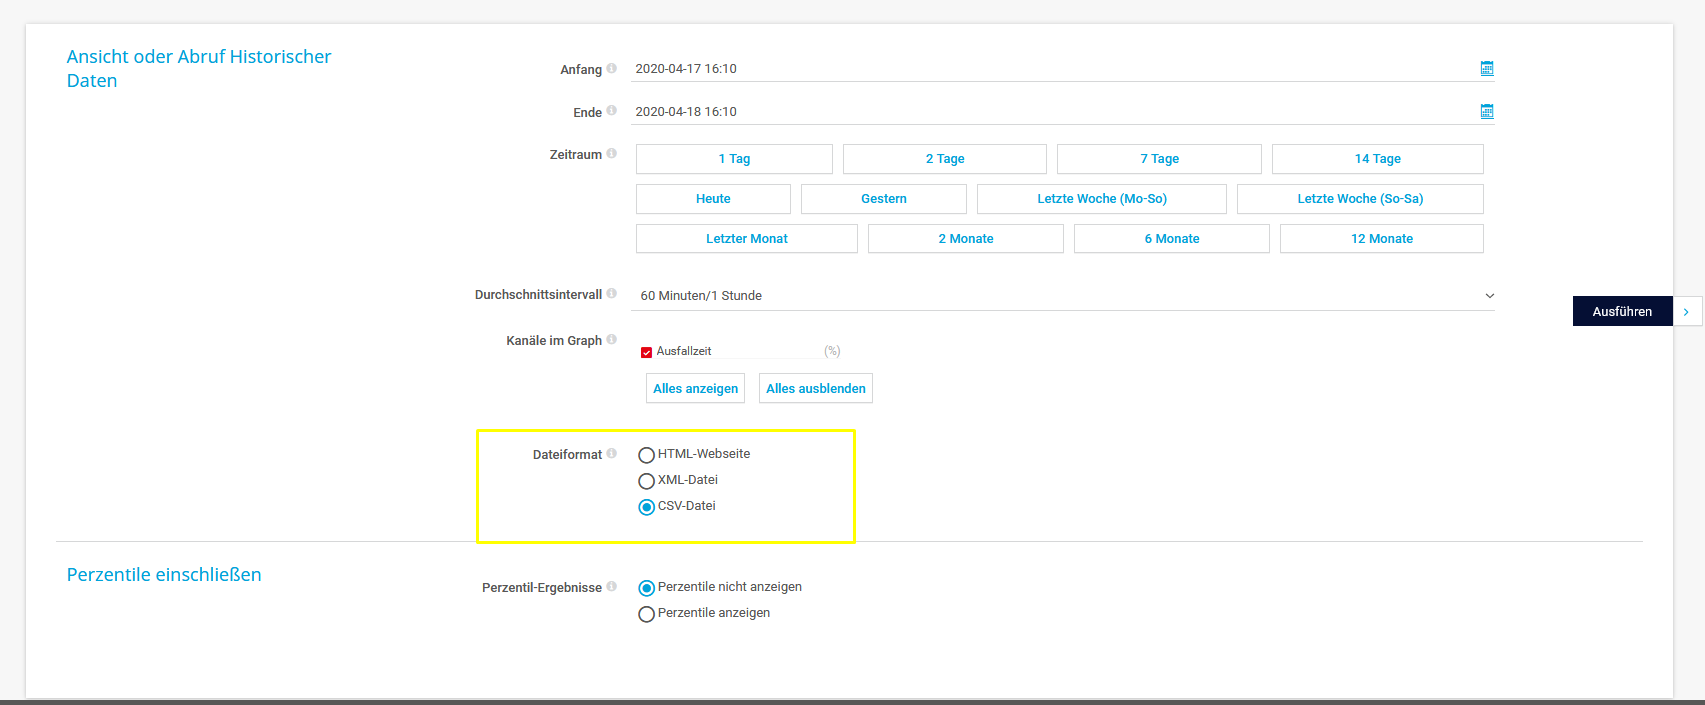
\includegraphics{./images/prtg-export.png}
\caption{PRTG Export von Daten}
\end{figure}

Mittels Excel können die Daten dann aufbereitet und weiterverarbeitet
werden, sofern man das möchte. Wir haben zur Veranschaulichung ein
Diagramm (Abbildung \ref{prtg-dia}) über die Performance der ReST-API
erstellt.

\begin{figure}[!htb]
\centering
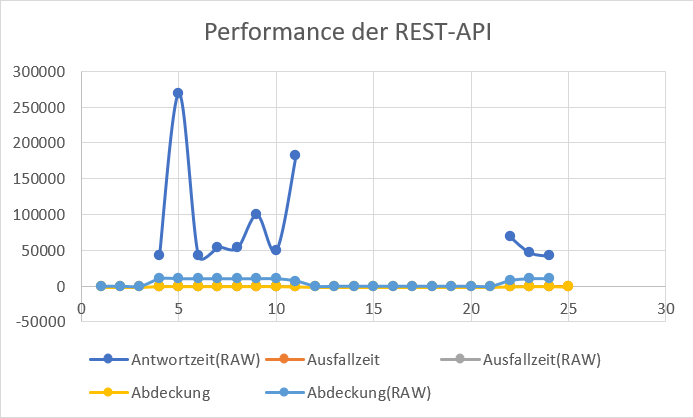
\includegraphics{./images/prtg-excel-stat.png}
\caption{PRTG REST-Performance Diagramm}\label{prtg-dia}
\end{figure}

Mit PRTG ist es auch möglich über eine SSH-Session, Informationen über
einen Server auszulesen wie z.B. die verfügbare Speicherauslastung.

\begin{figure}[!htb]
\centering
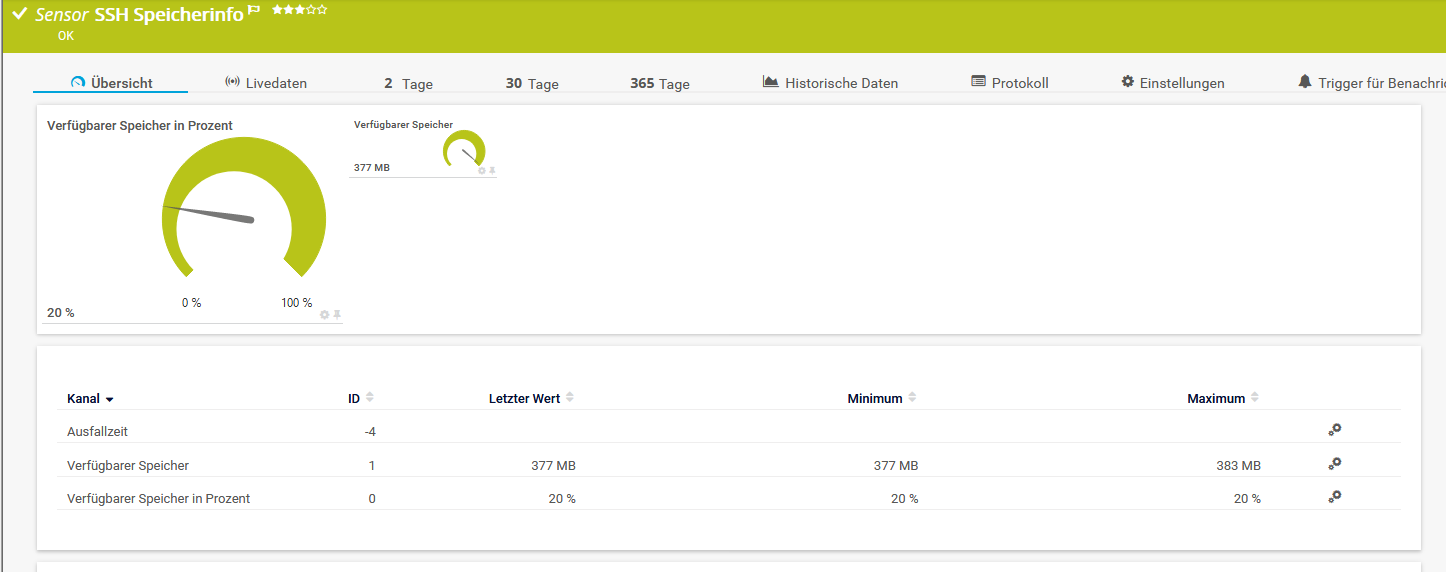
\includegraphics{./images/prtg-ssh-speicher.png}
\caption{PRTG SSH-Speicherauslastung}
\end{figure}

\hypertarget{uxfcberwachung-windows-server}{%
\subsection{Überwachung Windows
Server}\label{uxfcberwachung-windows-server}}

Die Überwachung eines Windows-Servers geht ein wenig anders von statten.
Hier findet der Informationsaustausch über
WMI\(\footnote{Windows Management Instrumentation}\), Performance
Counters oder SNMP statt. Die Vorteile bei SNMP liegen darin, dass es
eine deutlich geringere last verursacht, als seine Microsoftproprietären
Alternativen. Damit eht jedoch einher, dass WMI und Performance Counters
eine größere Menge an Daten anbieten, was bei einer rundum Überwachung
das um und auf ist.

In unserem Fall werden wir Log-Datein über de Windows Management
Instrumentations auswerten und einen modifizierten Sensor erstellen, der
bei dem Überschreiten eines Schewellenwertes ein Ticket erstellt.
Genauer der Ordner Desktop bei dem ab 4 Files ein neues Ticket erstellt
wird.

Im ersten Schritt muss der Sensor hinzugefügt werden. Dazu dem
vorherigen Prozedere folgen. Danach im Reiter \emph{Trigger für
Benachrichtigungen} ein neuer \emph{Schwellenwerttrigger} hinzugefügt
werden.

\begin{figure}[!htb]
\centering
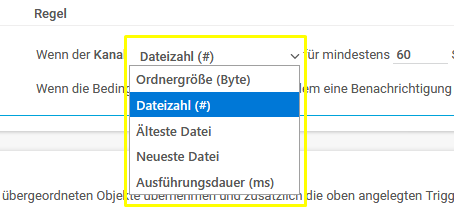
\includegraphics{./images/prtg_kanal.png}
\caption{PRTG Dateikanäle}
\end{figure}

Wenn man nun einige Dateien erstellt und ein wenig wartet erscheint
unter dem \emph{Tickets} Reiter ein neues Ticket:

\begin{figure}[!htb]
\centering
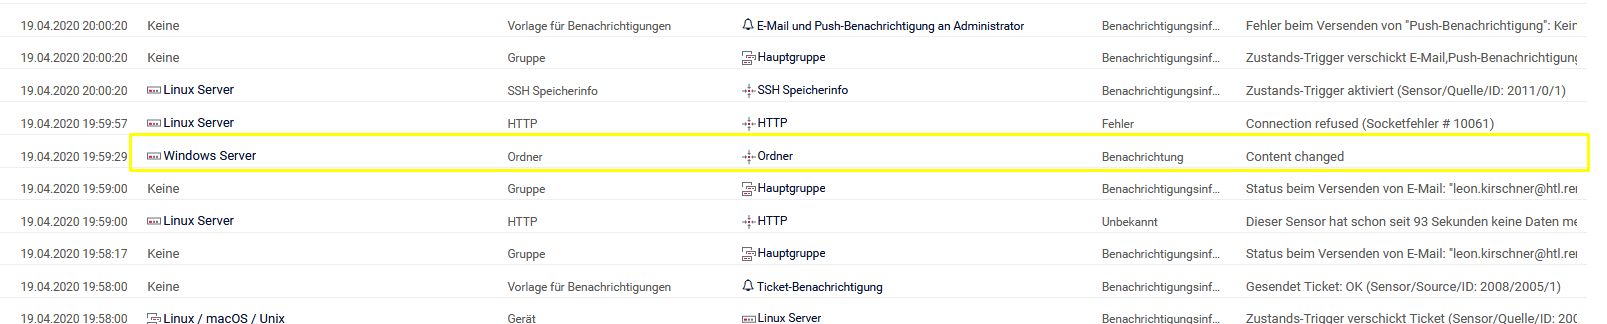
\includegraphics{./images/prtg-ticket-folder.png}
\caption{PRTG Schwellenwertfolder}
\end{figure}

\hypertarget{lessons-learned}{%
\section{Lessons Learned}\label{lessons-learned}}

Die Arbeit und das erkunden mit PRTG hat uns viel Spaß gemacht. Da
unsere VMs in der Schule zwei mal gelöscht wurden, ging jedoch leider
viel Zeit für die Windows- bzw. Linux Installation drauf, die wir gerne
in PRTG investiert hätten. Nichtsdestotrotz ist unser Fazit, dass PRTG
ein sehr mächtiges - wenn auch teures - Tool zur Überwachung eines
Netzwerkes ist. Der große Unterschied zu seinen (Open Source)
Konkurenten wie Nagios, wirbt es damit, keine Plugins anzubieten weil es
standardmäßig alles kann. Auch wenn wir nicht alles im Protokoll
vermerken konnten sind wir der Meinung, dass PRTG seinem Ruf gänzlich
gerecht wird. Durch das intuitive Web-UI ist es auch möglich, relativ
schnell und ohne viel Vorwissen Sensoren hinzuzufügen und ein IT-System
überwachen kann.
 

\end{document}